\label{chap-intro}

This chapter introduces the topics that will be addressed in the first six chapters regarding finite area smoothing. First, \secref{intro-GAM} gives an introduction to smoothing using splines in two dimensions, \secref{intro-extending} then discusses the larger class of models to which the smoothers belong, \secref{intro-inpractice} addresses some more practical issues, then finally \secref{intro-FAS} goes on to talk about existing approaches to spatial smoothing in a finite area.

\section{Smoothing in two dimensions using splines}
\label{intro-GAM}

In ecological studies, it is typical that one of the covariates collected is the location at which the sample has been taken. Two possible uses for such data are considered here. First, location may be the only covariate collected, in which case estimating the spatial distribution of the phenomena in question is the goal (usually by plotting some kind of surface as a function of geographical coordinates). Alternatively, the spatial covariates may be used to remove spatial autocorrelation from the data, making the effects of non-spatial covariates clear and thus improving inference.

The following two examples highlight these two different objectives:
\begin{enumerate}
\item Chlorophyl levels in the Aral sea are monitored using satellite images. Each pixel in the image represents an area of 9 kilometres square on the Earth. However, the satellite images are noisy and so adjacent pixels can have vastly different measured levels of chlorophyll. One would expect the levels to vary smoothly with location, so a model can be fitted to the image data which produces a smooth map of the chlorophyll concentration over the whole of the sea in an attempt to remove the noise. Figure \ref{aral-intro} shows both raw and smoothed chlorophyll levels in the Aral sea (these data are revisited in section \ref{aral-sec} and \ref{aral-revisit}).
\item We wish to model the distribution of the North sea whiting population through space and time. In particular numbers of fish of age one were recorded by pulling a net up through the water column at a set of sample points. The sample locations and dates were recorded along with sea surface temperature, the identity and nationality of the ship that took the measurement and the depth of the sea bed at the sample location. Such a model can be used to draw inference about how the population has changed over time (for example, to see if overfishing is a problem or perhaps to see if there are reporting discrepancies between ships). The whiting's distribution in space and time is non-homogeneous (in particular it is known that yearlings tend to be found close to the shore) and failing to model this spatial heterogeneity could introduce  bias in abundance estimates. Accurately modelling the spatial distribution is essential for reliable inference.
\end{enumerate}
In both of these examples it is assumed that the phenomena in question (chlorophyll concentration and whiting density) vary smoothly according to their spatial location in the sense that the trend surface does not have large jumps as location changes. In many situations this assumption is biologically plausible.

% Aral example
\begin{figure}[tb]
\centering
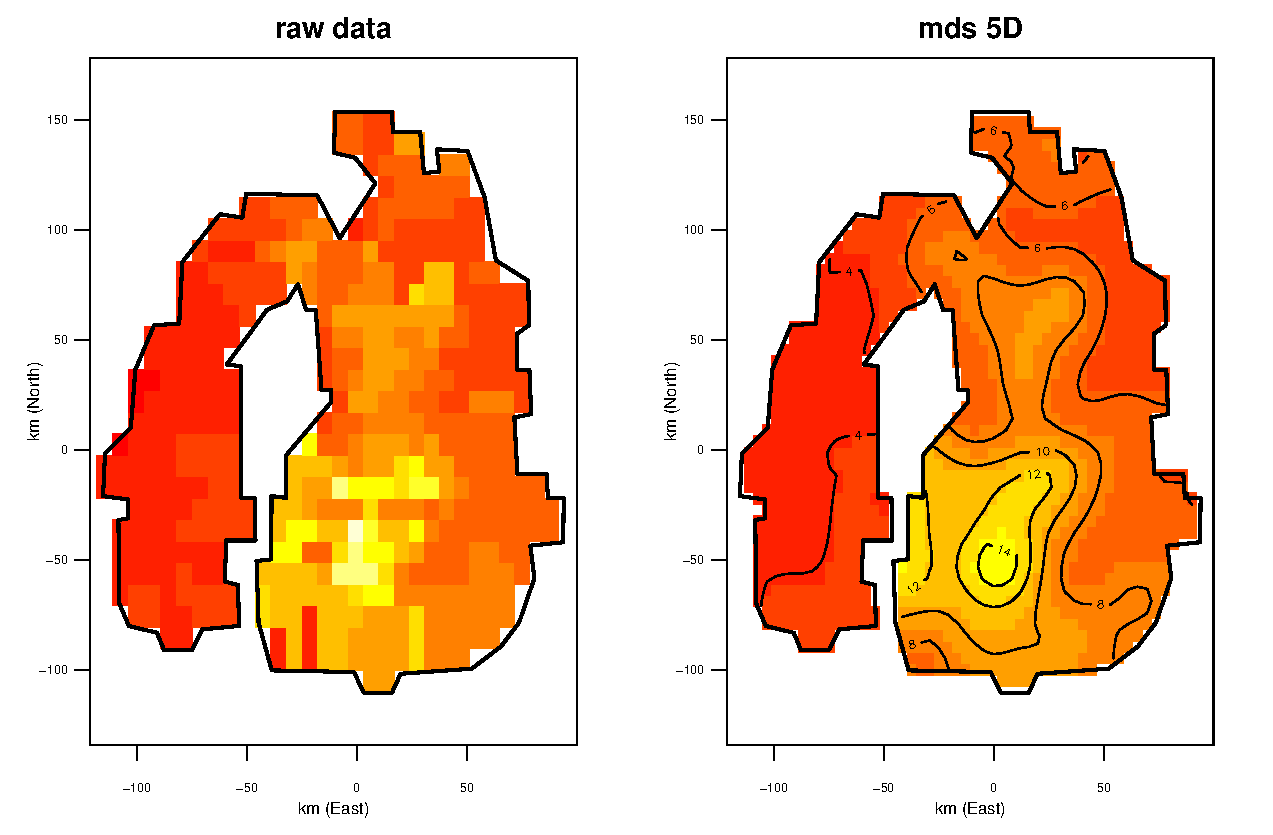
\includegraphics[width=\textwidth]{mds/figs/aral-5d-duchon.pdf}\\
\caption{Left: raw chlorophyll levels in the Aral sea as recorded by the SeaWIFS satellite. Right: a smoothed version of the data. Further analysis of the data may be found in sections \ref{aral-sec} and \ref{aral-revisit}.}
\label{aral-intro}
\end{figure}

There are many ways to construct models for the data described in the above examples, popular methods include kriging (\cite{diggle},  \cite{schabenberger}), kernel density estimation (\cite{wandKDE}) and hierarchical Bayes models (\cite{banerjee}). Here the focus is on using \textit{splines} (e.g. \cite{wahba}) for spatial smoothing via \textit{additive models} (e.g. \cite{gammonograph}).

Of particular interest here are smooth functions of space, and since the models are additive the emphasis is on situations akin to example 1 above, since if a method can be used in this context, it can also be included in models like those in example 2, simply as an additive component. For this reason, non-spatial covariates are ignored (for now).

Chapter 2 illustrates a situation akin to example 1 using administrative data from Italy and is based on the work in \citeb{miller2011}.

\subsection{Basic setup}
\label{intro-basic-setup}

First, denote observations of the phenomenon of interest as $z_i$ (in the examples above this would be the chlorophyll level or the yearling whiting catch at a particular point); $i$ indexes the samples $i=1,\ldots,n$, if there are $n$ samples . Each  $z_i$ is the realisation of some random variable $Z_i$, where $Z_i=\mu_i+\epsilon_i$, where $\mu_i=\mathbb{E}(Z_i)$, the expected value of the $i^\text{th}$ observation. Here $\epsilon_i$ is an error term and is assumed to be normally distributed with zero mean and some variance, $\sigma^2$. The spatial coordinates of the sample are also recorded, denote them $\mathbf{x}_i = (x_{i1}, x_{i2})$ (coordinates could be measured in latitude and longitude, or as kilometres North and East of some reference point, known as Northings and Eastings). The objective is to model the expected value of the response ($\mu_i$) using the coordinates at which the data were collected.

Assuming that the phenomenon of interest varies smoothly in space is equivalent to saying that $\mu_i$ varies smoothly in space. Letting $f$ be some smooth function, then as $\mu_i = f(\mathbf{x}_i)$:
\begin{equation*}
z_i = f(\mathbf{x}_i) + \epsilon_i.
\end{equation*}
The observations are a sum of a smoothly varying spatial component and some random error. The problem is now how to estimate $f$.

One can imagine several possible ways of obtaining a suitable $f$. For example, one might simply work through a large book of mathematical functions, estimating parameters and finding the function that would fit the data best (for some definition of ``best''). Alternatively one might estimate $f$ as a kind of moving average of the values (for example LOESS, \cite{loess2}). The first option seems extremely time consuming (if it were even plausible) and the second will not give an ``explicit'' functional form at the end to slot into other procedures later. Rather than use either of these, a \textit{basis function} representation is used for $f$. The idea is to build $f$ out of a sum of $J$ known functions, ($b_j$s, say) scaled by coefficients ($\beta_j$, say) and then estimate these coefficients rather than the function as a whole. Mathematically:
\begin{equation}
 f(\mathbf{x}_{i}) = \sum_{j=1}^J \beta_j b_j(\mathbf{x}_{i}).
\label{intro-basisdecomp}
\end{equation}
Now some care must be taken in choosing both how many $b_j$s are used ($J$) and their form. This is so that $f$ sufficiently flexible over the whole of the domain that is to be smoothed over. 

The next few sections present a brief introduction to how spatial smoothing using splines works, with a particular emphasis on the spatial case. However, it should be noted that at all times the models presented can be extended to higher (and lower dimensions) and that two dimensions are used for clarity and relevance. The primary references for the rest of this section are \citeb{simonbook} and \citeb{rwc}, both provide excellent complementary introductions to the topic.

\subsection{Smoothing with penalties}
\label{GAMpenalties}

If $f$ is very flexible it is possible that in estimating the $\beta_j$s an $f$ which tends toward interpolation of the data can be found. Interpolating the data is not useful since an $f$ that simply jumps from datum to datum does not say any more about the spatial distribution than merely looking at the data. To obtain an $f$ that interpolates the data, we can simply minimize the ordinary least squares (OLS) objective function. That is estimate the vector of coefficients, $\hat{\bm{\beta}}$, that minimizes:
\begin{equation}
\sum_{i=1}^n \left \{ z_i - f(\mathbf{x}_i) \right \}^2,
\label{intro-OLS}
\end{equation}
If the $b_j$s are a sufficiently rich set of functions, this objective function does nothing to stop $f$ simply interpolating the data (which would give a value of 0 in the above expression). To stop this from happening the ``wigglyness'' of $f$ is penalized.

Penalizing the \textit{wigglyness} (or \textit{roughness}, \cite{rwc}) of $f$ makes sense since (as stated above) the belief is that the underlying phenomena is smooth. Mathematically, taking (\ref{intro-OLS}) and adding on a penalty based on the wigglyness gives:
\begin{equation}
\sum_{i=1}^n \left \{ z_i - f(\mathbf{x}_i) \right \}^2 +  \lambda \int\int \lvert \lvert P f(\mathbf{x}) \rvert \rvert^2 \text{d}\mathbf{x}.
\label{intro-2d-objfcn}
\end{equation}
Here $P$ is some derivative operator, for example the second derivatives (e.g. $P=\left ( \frac{\partial^2}{\partial x_1^2}, \sqrt{2} \frac{\partial^2}{\partial x_1 x_2}, \frac{\partial^2}{\partial x_2^2}\right )$ in a 2-dimensional case). Integrating the derivatives over the whole space gives a measure of the wigglyness of the function, functions which vary a lot will lead to large values of the integral and hence have larger penalties. The exact form of $P$ changes with the basis and dimensionality of the problem (as will be seen in the next section).

Depending on the situation, the penalty should have a different amount of influence on (\ref{intro-2d-objfcn}). The \textit{smoothing parameter}, $\lambda$($\geq0$), controls the trade-off between interpolation (which happens as $\lambda \rightarrow 0$, leading to no penalty) and fitting a simpler function (which happens as $\lambda \rightarrow \infty$, where all terms are penalized aside from those for which the integral evaluates to zero: those in the \textit{nullspace} of the penalty). Figure \ref{lambda-ex} shows how different values of $\lambda$ affect the fitted smooth function. Determining the value of $\lambda$ will be covered in section \ref{GAMfitting}. For now it is assumed that some optimal $\lambda$ is known.

% example of setting lambda 
\begin{figure}[tb]
\centering
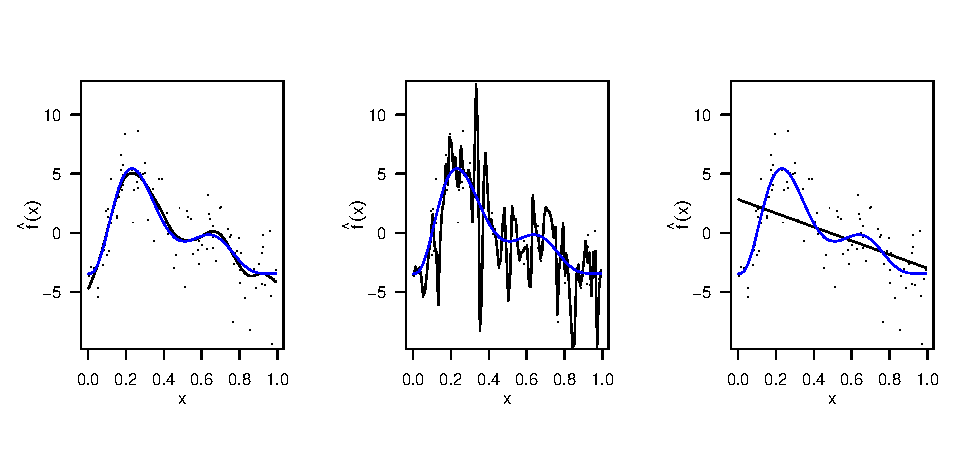
\includegraphics[width=6in]{intro/figs/lambda-ex.pdf}\\
\caption{An example of how different values of $\lambda$ affect the fitted smooth function of one variable. In the left panel, $\lambda$ is chosen optimally by GCV (see section \ref{GAMfitting}), in the middle panel $\lambda=0$, tending towards an interpolating fit. In the right panel $\lambda=\infty$ leading to a straight line. In each panel the blue curve is the true function and the points are the data sampled from it with error.}
\label{lambda-ex}
\end{figure}

The expression for the penalty given in (\ref{intro-2d-objfcn}) looks like it might require a rather large amount of integration and as such would require a long time to compute however, it can be shown (\cite[p. 128]{simonbook}) that the integral can be written as:
\begin{equation}
\int \dots \int \lvert \lvert P f(\mathbf{x}) \rvert \rvert^2 \text{d}\mathbf{x} = \bm{\beta}^\text{T} \mathbf{S} \bm{\beta},
\label{pen-quadform}
\end{equation}
where the $ij^\text{th}$ element of $\mathbf{S}$ is the integral of the product of the appropriate derivatives (in the above example, second) of the $i^\text{th}$ and $j^\text{th}$ basis functions. Put more mathematically:
\begin{equation*}
\mathbf{S}_{ij} = \int \dots \int \left(Pb_{i}(\mathbf{x})\right ) \left (Pb_{j}(\mathbf{x}) \right )^\text{T}  \text{d}\mathbf{x}.
\end{equation*}
So in this case the penalty matrix $\mathbf{S}$ only needs to be computed once. Computation of the penalty is merely a case of calculating the quadratic form in (\ref{pen-quadform}).

\subsection{Spline bases}

So far all that has been said about the form of $f$ is that it can be decomposed into a series of basis functions. Three bases are discussed here: \textit{thin plate regression splines}, \textit{P-splines} and \textit{cubic splines}, which will be used in this thesis.

\subsubsection{Thin plate regression splines}
\label{GAMtprs}
\label{GAMtprspenalty}

This section begins by discussing \textit{thin plate splines} before going on to describe a computationally efficient version of the basis (\textit{thin plate regression splines}) which will be used throughout the thesis. Thin plate splines are particularly useful in a spatial setting because they have a property known as \textit{isotropy}: all directions have a common smoothing parameter so wigglyness in the $x_1$ direction has the same weight in the penalty as in the $x_2$ direction (and so on through higher dimensions). This property is usually appropriate in a spatial setting, since there is nothing special about one geographical coordinate over another when it comes to the smoothness of the function to be fitted.

Thin plate splines were first proposed by \citeb{duchon77}. Duchon begins by presenting the following penalty:
\begin{equation}
J_{m,d} = \int \ldots \int_{\mathbb{R}^d} \sum_{\nu_1 + \dots + \nu_d=m} \frac{m!}{\nu_1! \dots \nu_d!} \left ( \frac{\partial^m f(x_1,\dots,x_d)}{\partial x_1^{\nu_1} \ldots  \partial x_d^{\nu_d}} \right )^2 \text{d} x_1 \ldots  \text{d} x_d,
\label{tprs-pen}
\end{equation}
where $m$ is the \textit{derivative order}, $d$ is the dimension of the data (in a spatial setting $d=2$) and the $\nu_1,\ldots,\nu_d$ terms simply ensure that derivatives are taken with respect to all the parameters in all of the necessary combinations.

Replacing the penalty in (\ref{intro-2d-objfcn}) with (\ref{tprs-pen}), the objective function is then:
\begin{equation*}
\sum_{i=1}^n \left \{ z_i - f(\mathbf{x}_i) \right \}^2 +  \lambda J_{m,d}
\end{equation*}
It can then be shown that this objective function is minimized by a function of the form:
\begin{equation}
f(\mathbf{x}) = \sum_{i=1}^n \delta_i \eta_{m,d}(r_i) + \sum_{j=1}^M \alpha_j \phi_j(\mathbf{x}),
\label{tprs-basis} 
\end{equation}
where $r_i=\lvert \lvert \mathbf{x}-\mathbf{x_i}\rvert \rvert$ (the Euclidean norm of $ \mathbf{x}-\mathbf{x_i}$) and the $\delta_i$s and $\alpha_j$ are parameters to be estimated. As in (\ref{intro-basisdecomp}), $f$ is decomposed into a sum of basis functions however, for a thin plate spline this summation is split into two parts: $M$ polynomials that act over the whole of the data (the $\phi_j$s) and a set of \textit{radial basis functions}, one centred at each datum (the $\eta_{m,d}$s). One can think of this as a global trend (in the 2-dimensional case, linear functions of the two coordinates) with extra flexibility provided by the radial basis functions.

The radial basis functions $\eta_{m,d}(r)$ are defined as:
\begin{align*}
\eta_{m,d}(r) =\begin{cases} \frac{(-1)^{m+1+d/2}}{2^{2m-1}\pi^{d/2}(m-1)!(m-d/2)!} r^{2m-d} \log(r) &\quad{\text{$d$ even,}}\\
\frac{\Gamma(d/2-m)}{2^{2m}\pi^{d/2}(m-1)!} r^{2m-d} &\quad{\text{$d$ odd.}}
\end{cases}
\end{align*}
where $\Gamma$ is the gamma function. The $\phi_j$s are $M=\left( \begin{smallmatrix} m+d-1 \\ d  \end{smallmatrix}\right)$ linearly independent polynomials of degree less than $m$ which span the space of polynomials in $\mathbb{R}^d$; all of the $\phi_j$s are unpenalized as they lie in the nullspace of the penalty. It is also important to note that to maintain continuity in $f$, $2m>d$; this means that the dimension of the nullspace increases rapidly with $d$ (this will be discussed further in chapter \ref{chap-gds}).

This all looks rather complex, however in the 2-dimensional case, (\ref{tprs-pen}) looks much simpler. Setting $d=2$ and $m=2$, (\ref{tprs-pen}) is given as:
\begin{equation*}
J_{2,2} = \int \int \left ( \frac{\partial^2 f(x_1,x_2)}{\partial x_1^2} \right )^2 + 2\left ( \frac{\partial^2 f(x_1,x_2)}{\partial x_1  \partial x_2} \right )^2 + \left ( \frac{\partial^2 f(x_1,x_2)}{\partial x_2^2} \right )^2 \text{d} x_1 \text{d} x_2,
\end{equation*}
and $f$ is:
\begin{equation*}
f(\mathbf{x}) = \sum_{i=1}^n \delta_i \eta_{2,2}(r_i) + \sum_{j=1}^3 \alpha_j \phi_j(\mathbf{x}),
\end{equation*}
where:
\begin{equation*}
\eta_{2,2}(r) = \frac{1}{8\pi} r^2 \log(r).
\end{equation*}
The nullspace of the penalty consists of three functions: $\phi_1(\mathbf{x})=1, \phi_2(\mathbf{x})=x_1 \text{ and } \phi_3(\mathbf{x})=x_2$, which make no contribution to $J_{2,2}$. Figure \ref{tprs-basis-fig} shows some examples of 2-dimensional thin plate basis functions.

% tprs basis fig
\begin{figure}[p]
\centering
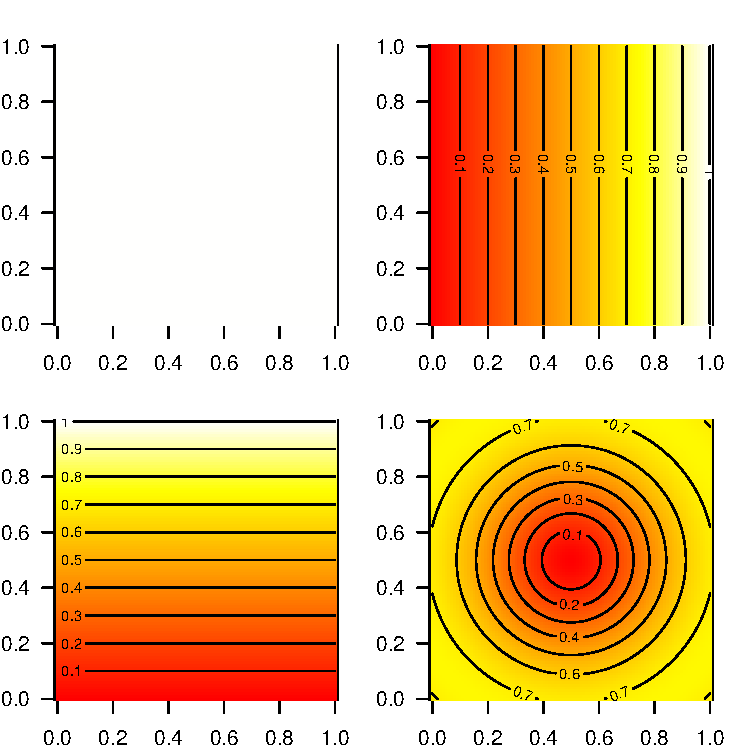
\includegraphics[width=\textwidth]{intro/figs/tprsex.pdf}\\
\caption{Example of a thin plate spline basis. The first three are $\phi_1(\mathbf{x})=1, \phi_2(\mathbf{x})=x_1 \text{ and } \phi_3(\mathbf{x})=x_2$, which are in the nullspace of the $J_{2,2}$ penalty. The bottom right plot shows an example of a radial basis function centred on $(0.5,0.5)$ with coefficient $-100$ (to put it on the same colour scale).}
\label{tprs-basis-fig}
\end{figure}

The computational cost of fitting the model is cubed in the number of parameters, so fitting a model with one radial basis function per datum may prove impractical in some cases. To avoid this problem, one could either ($i$) select (perhaps randomly) some of the data and use only those points to create the basis and then use the full data to fit the model (i.e. changing the index of the summation in the first term of (\ref{tprs-basis})) or ($ii$) select a (relatively small) representative set of points within the space covered by the data (though not necessarily data locations) which would be evenly spread out enough to create the basis (changing the $\mathbf{x}_i$s in the first summation in (\ref{tprs-basis}) -- these points are known as \textit{knots}). Both approaches have potential problems, namely: how many points should be chosen and where they should best be located? Both of theses approaches effectively reduce the size of the basis (changing the limit on the first summation in (\ref{tprs-basis})), however both methods do this in a fairly arbitrary way. There is no objective measure of whether the points selected are ``good''. 

\citeb{wood2003} proposes a low-rank approximation to thin plate splines, referred to in this thesis as \textit{thin plate regression splines}. Let the $ij^\text{th}$ element of the ($n \times n$) matrix $\mathbf{E}$ be the $j^\text{th}$ radial basis function evaluated at the $i^\text{th}$ datum (i.e. $\mathbf{E} = \eta_{m,d}\left (\vert\vert\mathbf{x}_i - \mathbf{x}_j \vert\vert \right )$), reducing the computations required to fit the model can be achieved by reducing the rank of $\mathbf{E}$. In the previous two approaches the rank reduction was performed by removing columns from $\mathbf{E}$ (randomly sampling the data) or changing the number of columns by changing the location of the evaluations (using knots). 

One way of reducing the size of $\mathbf{E}$ is by performing an eigen-decomposition (so $\mathbf{E}=\mathbf{U}\mathbf{\Lambda}\mathbf{U}^\text{T}$, where the columns of $\mathbf{U}$ are orthogonal eigenvectors and $\mathbf{\Lambda}$ is a diagonal matrix of eigenvalues decreasing in absolute value down the diagonal). Picking the $k$ largest eigenvalues and truncating at that point (taking the first $k$ columns of $\mathbf{U}$ and the top right $k\times k$ submatrix of $\mathbf{\Lambda}$) gives $\mathbf{E}_k(=\mathbf{U}_k\mathbf{\Lambda}_k\mathbf{U}_k^\text{T})$. It can be shown that the reduced rank matrix $\mathbf{E}_k$ gives the best approximation to $\mathbf{E}$ (see \cite{wood2003} for details). In practice, $k$ is set to be ``large enough'' and further reduction in basis complexity is performed by penalization (see \secref{GAMEDF}). In the simulations and analyses in the following chapters $k$ will be referred to as the ``maximum basis size'' to avoid confusion.

This low-rank approximation is the default implementation when using the ``\texttt{tp}'' basis in the \textsf{R} package \texttt{mgcv}. This package was used throughout the thesis.

\subsubsection{P-splines}
\label{intro-psplines}

P-splines (\cite{eilersmarx96}) consist of B-spline basis function with discrete penalties, so before thinking about P-splines, the properties of B-splines are considered. 

B-splines are simple local basis functions; they are simple in that all of the basis functions have the same shape and local in that they only have an effect near where they are centred (at the knots) -- \textit{compact support}. Taking (\ref{intro-basisdecomp}), we replace the $b_j$s with an $(m+1)^\text{th}$ order B-spline $B_j^m$ (where the order is chosen). Note that the $B_j^m$s are only a function of one covariate, $x$, at this point but will be expanded to higher dimensions below. So, the basis representation of $f$ given in (\ref{intro-basisdecomp}) becomes:
\begin{equation*}
f(x) = \sum_{j=1}^{J} \beta_j B^m_j(x).
\end{equation*}
The $B_j^m$s are defined recursively as:
\begin{equation*}
B_j^m(x) = \frac{x-x^*_j}{x^*_{j+m+1} - x^*_j} B_j^{m-1}(x) + \frac{x^*_{j+m+2} -x}{x^*_{j+m+2} - x^*_{j+1}} B_{j+1}^{m-1}(x) \quad \text{for } j=1,\ldots,J,
\end{equation*}
and
\begin{equation*}
 B_j^{-1}(x)=\begin{cases}
1 \quad x_j \leq x < x_{j+1}\\
0 \quad \text{otherwise}. 
\end{cases}
\end{equation*}
The $J+m+1$ knots $x^*_j$ are evenly spaced over the $x$-axis and these, along with the order of the basis, determine how flexible $f$ is. Each $B^m_j(x)$ is non-zero over the $m+3$ adjacent knots. Contrary to their rather complex functional form, the functions shown in figure \ref{bs-basis} are rather simple. From left to right the panels show B-splines bases with $m=1,2,3$ for evenly spaced knots over $(0,1)$.

% b-splines example 
\begin{figure}[tb]
\centering
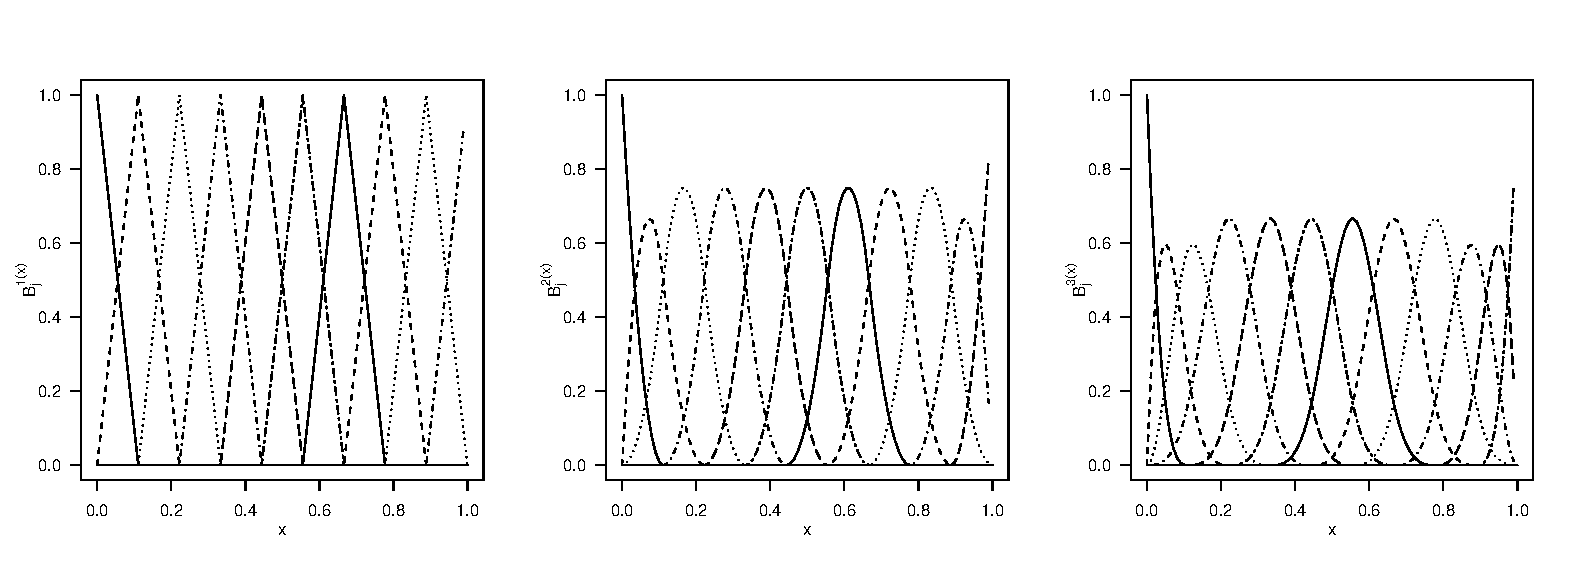
\includegraphics[width=\textwidth]{intro/figs/bspline-ex.pdf}\\
\caption{An example of B-spline basis functions for $m=1, 2$ and $3$ (from left to right) with evenly spaced knots (these are located at the peaks of the basis functions).}
\label{bs-basis}
% generated by phd-smoothing/thesis/intro/figs/bspline-ex.R 
\end{figure}

P-splines take the B-spline basis and add a penalty structure. Because of their local nature, the penalty is somewhat different to the general penalty in (\ref{intro-2d-objfcn}) and is based on differences between adjacent bases. Since the $B^m_j$s are defined locally, smoothness only needs to be enforced on neighbouring basis functions. The objective function given in (\ref{intro-2d-objfcn}) then becomes:
\begin{equation*}
\sum_{i=1}^n \left \{ z_i - f(x_i) \right \}^2 +  \lambda \sum_{j=1}^{J-1} (\beta_{j+1} - \beta_j)^2,
\end{equation*}
if squared second differences are used (this could be a higher order difference, see \cite{eilersmarx96}). Such a penalty is very fast to compute, since many of the elements of the penalty matrix, $\mathbf{S}$, are zero due to the local nature of the basis functions.


\subsubsection{Cubic splines}
\label{intro-cubic}

\textit{Cubic splines} are another a univariate basis and, like P-splines they require the specification of knots. Cubic splines are made up of sections of cubic polynomials which are continuous (up to second derivatives) at the joins. The objective function for a cubic spline is:
\begin{equation*}
\sum_{i=1}^n \left \{ z_i - f(x_i) \right \}^2 +  \lambda \int_{x^*_1}^{x^*_J}\left( \frac{\partial^2 f(x)}{\partial x^2} \right)^2 \text{d}x,
\end{equation*}
where $\{x_j^* : j=1,\ldots,J\}$ are $J$ knots. This gives rise to the set of cubic polynomials that form the basis. Such a basis has many possible parametrizations; here the ``cardinal'' parametrisation is used (the basis functions take the value one at one knot and zero at all others). The parametrization gives the following form for $f$:
\begin{align*}
f(x) =& \frac{x_{j+1}^* - x}{x_{j+1}^* - x_j^*} \beta_j + \frac{x - x_j^*}{x_{j+1}^* - x_j^*} \beta_{j+1}\\
& + \left\{ \frac{\left (x_{j+1}^* - x\right )^3}{x_{j+1}^* - x_j^*} - (x_{j+1}^* - x_j^*)(x_{j+1}^* - x)\right \}\frac{\delta_j}{6}\\
& + \left\{ \frac{\left (x - x_j^*\right )^3}{x_{j+1}^* - x_j^*} - (x_{j+1}^* - x_j^*)(x - x_j^*)\right \}\frac{\delta_{j+1}}{6} \qquad \text{if } x_j^* \leq x \leq x_{j+1}^*.
\end{align*}
Letting $\beta_j = f(x_j^*)$ and $\delta_j = \frac{\partial^2 f(x)}{\partial x^2}\vert_{x=x_j^*}$, one can then write the $\delta_j$s as a function of the $\beta_j$s. Summing over $j$ then yields an implicit set of $J$ $b_j$s as in (\ref{intro-basisdecomp}). The cubic spline basis is then parameterized in terms of its values (and the values of its derivatives) at the knots. This setup may seem odd but does lead to the spline having directly interpretable parameters (which is not the case for, say, thin plate splines). An example of a basis function is given in figure \ref{cs-basis}.

Further details may be found in \citeb[pp. 122-126, pp. 149-151]{simonbook}.

% cubic example 
\begin{figure}[tb]
\centering
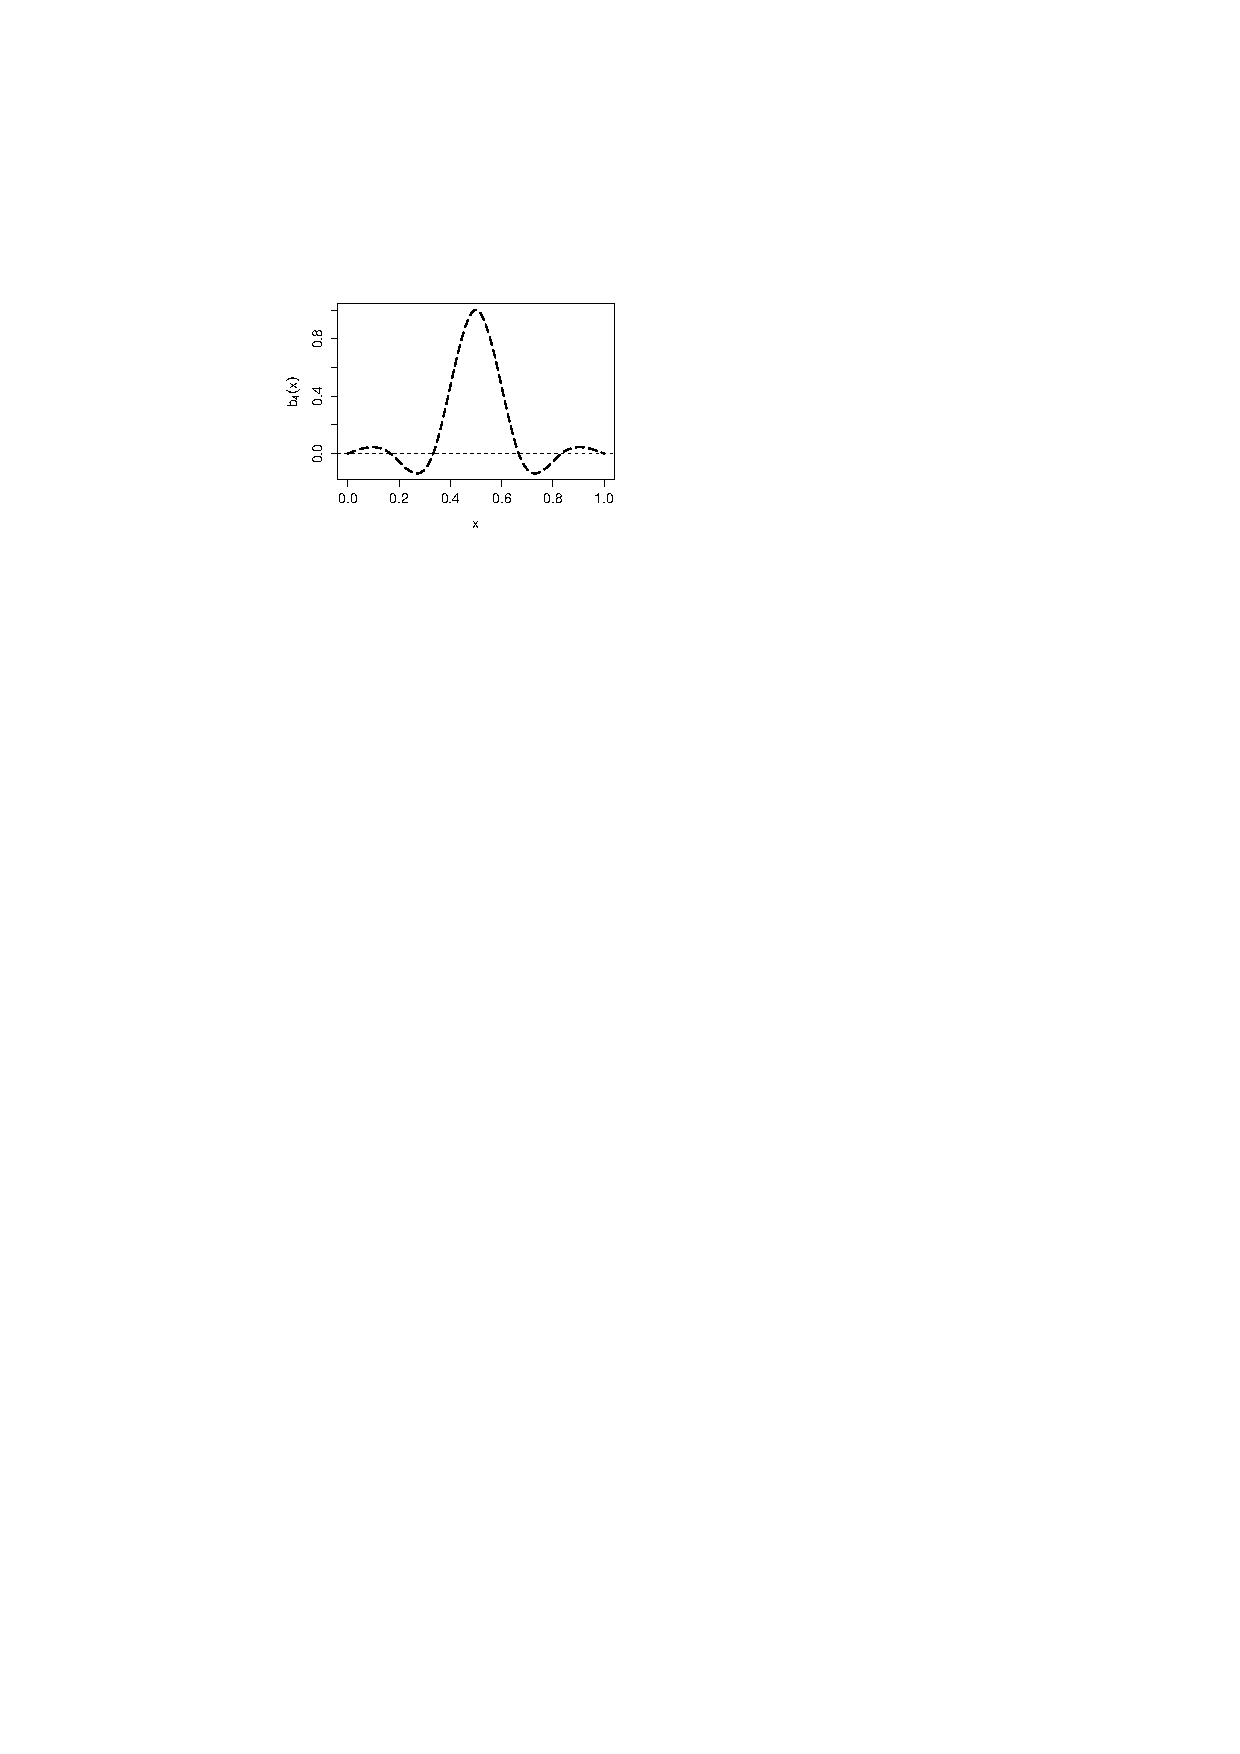
\includegraphics[width=0.5\textwidth]{intro/figs/cubic.pdf}\\
\caption{An example of a cubic spline basis function with a knot at 0.5. Figure taken from \citeb[p. 151]{simonbook}.}
\label{cs-basis}
% STOLEN! 
\end{figure}

\subsubsection{Cyclic cubic splines}

The above spline basis may be extended to a \textit{cyclic cubic spline} by imposing the constraint that $f(x_1)=f(x_k)$ and that the values of the first and second derivatives must also match. This specifies that the spline must ``join up'' at each end. The form of $f$ is the same as before, but there is one less coefficient to estimate (since the first and last are the same).

\subsubsection{Tensor products}
\label{GAMtensor}

Both P-splines and cubic splines are defined only in one dimension, however, it is possible to build 2-dimensional (and higher) smooths from \textit{tensor products} of 1-dimensional bases. This is made possible by thinking of each 1-dimensional basis as a marginal of the higher dimensional smooth. A spatial smooth of, say $x_1$ and $x_2$ can be constructed by first writing down the basis expansions for the marginal smooths of $x_1$ and $x_2$ (in general terms, since this applies to all splines not just P-splines and cubic splines, see \secref{3D}):
\begin{equation}
f_{x_1}(x_1) = \sum_{j=1}^J \beta_j b_j(x_{1}), \quad  f_{x_2}(x_2) = \sum_{k=1}^K \delta_k d_k(x_{2}).
\label{intro-tensor-def}
\end{equation}
where the $\delta_k$ and $d_k$ are analogous to $\beta_j$ and $b_j$ and assuming basis sizes of $J$ and $K$ (of course, $J$ and $K$ may be the same size). To make $f_{x_1}$ vary with $x_2$ we can then simply make the $\beta_j$s a function of $x_2$, the simplest way of doing this would be to define:
\begin{equation*}
\beta_j(x_2) = \sum_{k=1}^K \delta_{jk} d_k(x_{2}).
\end{equation*}
so then $f_{x_1,x_2}$ would is defined as:
\begin{equation*}
f_{x_1, x_2}(x_1,x_2) = \sum_{j=1}^J \sum_{k=1}^K \delta_{jk} d_k(x_{2}) b_j(x_{1}).
\end{equation*}
Finally, the penalty for such a smooth can be written:
\begin{equation*}
%\lambda_{x_1} \int\int \left \{P_{x_1} f_{x_1, x_2}(x_1,x_2)\right \}^2 \text{d}x_1\text{d}x_1 + \lambda_{x_2} \int\int \left \{P_{x_2} f_{x_1, x_2}(x_1,x_2)\right \}^2 \text{d}x_1\text{d}x_1,
\int\int \lambda_{x_1} \left \{P_{x_1} f_{x_1, x_2}(x_1,x_2)\right \}^2 + \lambda_{x_2} \left \{P_{x_2} f_{x_1, x_2}(x_1,x_2)\right \}^2 \text{d}x_1\text{d}x_2,
\end{equation*}
where $P_{x_1}$ and $P_{x_2}$ are derivative operators with respect to $x_1$ and $x_2$ respectively (or the equivalent discrete penalty in the P-spline case).

Although only a very simplistic example is given here, tensor product splines provide an extremely useful tool, allowing for extra dimensions to be added to models using different bases. The use of a different smoothing parameter for each direction allows for \textit{anisotropic} smoothing, so that covariates that are measured on different scales (for example temperature and length) may be combined into one tensor product smooth, avoiding the assumption that the degree of smoothing required is the same in both directions. In particular this can be useful when constructing a spatiotemporal smooth: for example using a thin plate spline for the spatial part of the smooth (so the spatial part of the model is isotropic) then taking a tensor product of that with a cubic spline basis (or another 1-dimensional thin plate spline) for the temporal effect (so a different amount of smoothing can be used for each direction). This is the setup that will be used in chapter \ref{chap-it} for the Italian data.

\subsection{Smoothing parameter selection by GCV}
\label{GAMfitting}

The objective function given in \secref{GAMpenalties} only allows the estimation of $\bm{\hat{\beta}}$ for some given $\lambda$ (or $\bm{\lambda}$); finding an optimal smoothing parameter has not yet been addressed.  A simple and effective way to find $\hat{\lambda}$ is to assess how well the model performs on data which were not in the sample -- i.e. assessing the prediction error of the model. The \textit{leave-one-out cross validation} score (LOOCV, see \secref{DEFN-LOOCV}) does exactly this by fitting the model to all but one of the data and calculating the difference between the prediction of the excluded datum and its true value (LOOCV is also known as \textit{ordinary cross validation}, OCV). Rather than fitting $n$ models to the data (one for each excluded datum), the \textit{generalized cross validation} (GCV) score can be used, which can be written as follows, allowing for easy computation:
\begin{equation}
\mathcal{V}_g = \frac{n \lvert\lvert \mathbf{z} - \mathbf{\hat{f}}\rvert \rvert^2}{\left \{n-\text{tr}(\mathbf{A}) \right \}^2},
\label{intro-GCV}
\end{equation}
where $\text{tr}(\mathbf{A})$ indicates the trace of $\mathbf{A}$, the hat (or influence) matrix for the smoother (see \secref{GAMEDF}), $\mathbf{\hat{f}}=\left(f(\mathbf{x}_1), f(\mathbf{x}_2), \ldots, f(\mathbf{x}_n)\right)^\text{T}$ is the vector of fitted values for the model (i.e. evaluations of $\hat{f}$ at each of the data). Numerical minimization of $\mathcal{V}_g$ with respect to $\lambda$ (which enters $\mathcal{V}_g$ via $\mathbf{A}$) gives the optimal smoothing parameter ($\hat{\lambda}$). Further details are given in \citeb[pp.  134--137]{simonbook}. Details of how smoothing parameter selection and estimation of $\bm{\hat{\beta}}$ are combined into a fitting procedure are given in \secref{intro-extending-gams}.



\section{Extending to more complex models}
\label{intro-extending}

So far only smooths of two geographical coordinates with normal errors in the response have been discussed. This section gives an overview of some extensions to these models.

\subsection{Covariates}

Although in the above, the focus has been on including on geographical coordinates as explanatory variables, other covariates (or combinations of covariates) can be included in an additive way. The notation in (\ref{intro-2d-objfcn}) and (\ref{pen-quadform}) is simply extended in this case and all of the above results hold, simply by defining $f(\mathbf{x})=\sum_k f_k(\mathbf{x}^{(k)})$ for the $k$ smooth functions $f_k$ of corresponding covariates ($\mathbf{x}^{(k)}$). The smoother matrix $\mathbf{S}$ is replaced by $\mathbf{S}= \sum_k \lambda_k \mathbf{S}_k$ where each $\mathbf{S}$ corresponds to an $f_k$ and multiple smoothing parameters (the $\lambda_k$) must be estimated. With such additive models identifiability becomes an issue since each of the $f_k$ can only be found up to some additive constant (since one could add a value, $a$ to $f_1$, say and then subtract it from $f_2$ leading to the same model as if $a$ were not included). To get around this problem \textit{identifiability constraints} are used. By enforcing a sum to zero constraint on the value of each function at the observed covariates the model is sure to be identifiable. 

\subsection{Higher dimensional smooths}

As well as including covariates as additive components, they can also be included as extra dimensions via tensor products (or directly into the basis in the \tprs\ case). When using thin plate splines, the order of the derivatives in the penalty ($m$) can be changed. Indeed, it is required that the derivative order changes according to the number of dimensions that smoothing takes place in ($2m>d$). Using a derivative order that is too low can lead to a non-smooth $f$, which is clearly undesirable. Smoothing in high dimensions can be unreliable and numerically tricky but not impossible (as will be seen later in chapter \ref{chap-gds}).

\subsection{Generalized additive models}
\label{intro-extending-gams}

Up until now only additive models with normal errors have been considered. If other exponential family response distributions are used with the models described above, we call this a \textit{generalized} additive model (GAM)  and in that case we may model $\eta_i=g(\mu_i)$ where $g$ is a \textit{link function} (in the same sense as the GLM case, see \cite[p. 8]{GEEbook}) and $\eta_i$ is the linear predictor. In order to estimate $\bm{\hat{\beta}}$, the \textit{penalized iteratively re-weighted least squares} (PIRLS) algorithm must be used. 

To use PIRLS, one must first think of the GAM as a penalized GLM. Consider first the usual GLM model matrix $\mathbf{X}$. By appending the basis evaluations of each datum as columns of $\mathbf{X}$ (i.e. $\mathbf{X}:=\left ( \mathbf{X},\mathbf{X}^* \right )$, where the $ij^\text{th}$ element of $\mathbf{X}^*$ is  $b_j(\mathbf{x}_i)$), the smooth terms in the model can be included in the usual model matrix setup. The PIRLS algorithm is as follows (\cite[p. 138]{simonbook}):

First define $\eta_i = \mathbf{X}_i\bm{\beta}$ (where $\mathbf{X}_i$ is the $i^\text{th}$ row of $\mathbf{X}$) as the linear predictor such that $\mu_i = g^{-1}(\eta_i)$ and the variance function, $V(\cdot)$, such that $\text{Var}\left ( Z_i \right ) = \phi V(\mu^{[k]})$ ($\phi$ is the scale parameter, see \cite[p. 62]{simonbook}). At iteration $k$ the PIRLS algorithm is:
\begin{enumerate}
\item Given the current linear predictor estimate and mean response vectors ($\bm{\eta}^{[k]}$ and $\bm{\mu}^{[k]}$, respectively) calculate the diagonal weight matrix with the following elements:
\begin{equation*}
\mathbf{W}^{[k]}_{ii}  \propto \frac{1}{V(\mu_i^{[k]})g^\prime(\mu_i^{[k]})^2},
\end{equation*}
and the pseudodata:
\begin{equation*}
s_i = g^\prime(\mu_i^{[k]})^2(z_i-\mu_i^{[k]}) + \mathbf{X}_i\bm{\hat{\beta}}^{[k]},
\end{equation*}
stored in the $n$-vector $\mathbf{s}$. $g^\prime(\mu_i^{[k]})$ is the first derivative of the link function with respect to $\mu_i^{[k]}$.
\item Minimize
\begin{equation*}
\lvert \lvert \sqrt{\mathbf{W}^{[k]}} (\mathbf{s}^{[k]} - \mathbf{X}\bm{\beta})  \rvert \rvert^2 + \lambda \int \dots \int \lvert \lvert P f(\mathbf{x})\rvert \rvert^2 \text{d}\mathbf{x}
\end{equation*}
with respect to $\bm{\beta}$, giving $\bm{\beta}^{[k+1]}$ and hence allowing the calculation of $\bm{\eta}^{[k+1]}$ and $\bm{\mu}^{[k+1]}$.
\end{enumerate}
This procedure is iterated to convergence of $\bm{\beta}$ for the given smoothing parameter(s). Further information on IRLS in the GLM context can be found in chapter 1 of \citeb{GEEbook}.

The ``hierarchical'' optimisation method of \citeb{remlpaper} is used throughout this thesis to find $\bm{\hat{\beta}}$ and $\bm{\hat{\lambda}}$. That is: at each iteration a smoothing parameter is selected to optimize the (GCV) score, which in the generalized case is given by:
\begin{equation*}
\mathcal{V}_g = \frac{n D(\bm{\hat{\beta}})}{\left \{n-\text{tr}(\mathbf{A}) \right \}^2},
\end{equation*}
where $D(\bm{\hat{\beta}})$ is the model \textit{deviance} (defined as the saturated $\log$-likelihood minus the $\log$-likelihood, evaluated at the current parameter values, all multiplied by $2\phi$) (see \cite[p. 178]{simonbook}). This optimal $\bm{\lambda}$ then implies a set of model coefficients (the best $\bm{\beta}$ for that $\bm{\lambda}$) which are found using PIRLS, the algorithm then proposes a new $\bm{\lambda}$ based on the derivatives of $\mathcal{V}_g$ with respect to $\log \bm{\lambda}$ at this point (the $\log$ scale is used to ensure that $\bm{\lambda}$ remains positive). This continues until convergence.

\subsubsection{Other GAM fitting methods}
\label{intro-otherGAMfit}

It has been observed (\cite{reissogden}) that the GCV score can sometimes have problems with multiple minima (i.e. the optimisation can get stuck at a non-optimal $\lambda$). \citeb{reissogden} also show that GCV tends to give more variable estimates for the smoothing parameter(s). An alternative to minimizing the GCV score ($\mathcal{V}_g$) is to use a likelihood-based method such as approximate REML or ML, which are less prone to this problem (\cite{remlpaper}). The key to understanding restricted maximum likelihood or (marginal) maximum likelihood methods is the realisation that the estimates of the coefficients (the $\bm{\hat{\beta}}$) are the posterior modes of the distribution of $\bm{\beta}|\mathbf{z}$ if $\bm{\beta} \sim N(\mathbf{0}, \phi \mathbf{S}^-)$ (where $\mathbf{S}^-$ the generalized matrix inverse of $\mathbf{S}$ and $\phi$ is the scale parameter, as above). When the $\bm{\beta}$ are considered to be random variables, smoothing parameters can then be thought of as variance parameters and a marginal likelihood can then be formed (this is known as the \textit{random effects formulation}).  This likelihood can then be optimized with respect to $\lambda$ and put in the place of the GCV score ($\mathcal{V}_g$) in hierarchical procedure above. At each iteration the optimal $\bm{\beta}$ is found via PIRLS.

%\citeb[pp. 120-123]{rwc} provide an interesting discussion of automatic smoothing parameter selection. In particular they note that as the number of data increases ($n\rightarrow\infty$), GCV only slowly converges to finding the optimum smoothing parameter, this leads to higher variability in the estimates of the smoothing parameter(s). In general GCV tends to select more complicated functions than likelihood based methods leading to overfitting to the data (see \cite{remlpaper} and \cite{reissogden}). REML and ML on the other hand will tend to fit smoother functions. However, it is important to note that this is a manifestation of the variance--bias trade-off. GCV will lead to less biased but more variable fits whereas likelihood based methods will be less variable but more biased. It does not seem that there is a clear ``best'' method for selecting smoothness but rather that both methods are imperfect in different ways. These issues did not manifest themselves when performing the spatial smoothing, but there were hints of this happening in the non-spatial models (see \secref{gds-examples}).

\citeb[pp. 120-123]{rwc} provide an interesting discussion of automatic smoothing parameter selection. In conclusion they state that there is no clear ``best'' method for selecting smoothness but rather that both methods are imperfect in different ways. 

%These issues discussed above did not manifest themselves when performing the spatial smoothing, but there were hints of this happening in the non-spatial models (see \secref{gds-examples}).

%In particular they note that as the number of data increases ($n\rightarrow\infty$), GCV only slowly converges to the optimal smoothing parameter, this leads to higher variability in the estimates of the smoothing parameter(s). In general GCV tends to select more complicated functions than likelihood based methods leading to overfitting (see \cite{remlpaper} and \cite{reissogden}). REML and ML on the other hand will tend to fit smoother functions. 

%However, it is important to note that this is a manifestation of the variance--bias trade-off. GCV will lead to less biased but more variable fits whereas likelihood based methods will be less variable but more biased. 

There are many other ways of fitting GAMs, such as backfitting (\citeb{gammonograph}, see also \secref{gds-intro}), Markov chain Monte Carlo (MCMC, e.g. \citeb{fahrmeir2004}) or integrated nested Laplace approximations (INLA, \citeb{inla}). The hierarchical procedure of \citeb{remlpaper} (using either GCV or REML/ML) was chosen over these other methods for several reasons. Backfitting and MCMC are quite computationally expensive, especially when larger models are used (see \citeb{simonbook}, pp. 213-215 for why this is the case for backfitting). MCMC-type approaches can be improved by exploiting sparse bases (like P-splines) however, thin plate regression splines (and their nice properties like isotropy) cannot be used. INLA can be very fast, however when many terms are included it becomes computationally expensive (\citeb{inla} suggest more than 10 become problematic).

\citeb{ruppertreview} gives an overview of developments in the area of semiparametric regression in general during the 2003--2007 period.

\section{Smoothing in practice}
\label{intro-inpractice}

This final section deals with two topics not covered above: assessing model performance and the practical implementation of the methods detailed above.

\subsection{Mean squared error}
\label{intro-MSE}

Simulation studies will be used extensively to evaluate the proposed methods. In order to determine the performance of the methods, some metric must be chosen. Mean squared error (MSE) is a standard approach to assessing the performance of a model, in terms of its prediction error. The MSE of the fitted model $\hat{f}$ is defined as:
\begin{equation*}
\text{MSE}(\hat{f}) = \mathbb{E}\left [\left \{ \hat{f}(X) - f(X) \right \}^2 \right ],
\end{equation*}
which (if there are $n_p$ prediction points) can be estimated as:
\begin{equation}
\widehat{\text{MSE}}(\hat{f}) = \frac{1}{n_p} \sum_{i=1}^{n_p} \left \{\hat{f}(\mathbf{x}_i) - f(\mathbf{x}_i) \right \}^2,
\label{DEFN-MSE}
\end{equation}
where $f(\mathbf{x}_i)$ is the ``true'' values of $f$ at the prediction points, $\mathbf{x}_i$. In the spatial simulations in the coming chapters, the prediction points will be a relatively dense set of locations to test how well $\hat{f}$ models the true surface. 

To test to see if two models' MSEs are significantly different, a paired Wilcoxon signed rank test (e.g. \cite[pp.173-175]{wetherill}) is used to analyse the results from simulations. When MSE is mentioned from now on, it will be with reference to $\widehat{\text{MSE}}$ in (\ref{DEFN-MSE}).

\subsection{The Brier score}
\label{DEFN-brier}

The Brier score (\cite{brier50}) is useful when the response variable is binary (a more general version of the score for $m$-ary variables can also be used). In this case the probability of observations belonging to a particular class (0 or 1 in the binary case) is measured, so it makes sense to assess the model performance using the probabilities rather than just the classifications. The score is similar in form to the MSE:
\begin{equation}
\text{BS} = \frac{1}{n} \sum_{i=1}^{n} \left \{\hat{f}_p(\mathbf{x}_i)-z_i \right \}^2
\end{equation}
where subscript $f_p$ indicates that the functions return values on the probability scale, rather than on the  scale of the linear predictor. The $z_i$s are the $n$, $m$-chotomous data. The Brier score has the advantage of offering a more granular measure of the model errors, since probabilities will be continuous on $(0,1)$ rather than dichotomous (or $m$-chotomous) class predictions.

\subsection{Leave-one-out cross validation}
\label{DEFN-LOOCV}

When analysing non-simulated data (where the true values are unknown) it is still sometimes necessary to quantify the out-of-sample error in predictions. This can be achieved using leave-one-out cross validation (LOOCV). The LOOCV score is calculated as:
\begin{equation}
\text{LOOCV} = \frac{1}{n} \sum_{i=1}^n \left \{ \hat{f}^{-i}(\mathbf{x}_i) - z_i \right\}^2,
\end{equation}
where $\hat{f}^{-i}$ is the model fit to all of the data except the $i^\text{th}$, so one can think of the LOOCV score as a measure of fit to unseen data.

\subsection{Effective degrees of freedom}
\label{GAMEDF}

The hat or influence matrix, $\mathbf{A}$, is the matrix such that $\hat{\bm{\eta}} = \mathbf{A}\mathbf{z}$. It has the rather useful property that taking the trace of $\mathbf{A}$ ($\text{tr}(\mathbf{A})$) gives the \textit{effective degrees of freedom} (EDF) of the model. The EDF gives an measure of the complexity of the fitted model. The higher the EDF, the more complex the model. The rationale for this is by analogy to the linear model. In that case we know that the degrees of freedom is simply the length of $\bm{\beta}$ (minus any identifiability constraints) which is the same as the value of $\text{tr}(\mathbf{A})$ if the smoothing parameters are all set to zero. It can also be shown that the minimum value of the EDF is $\text{rank}(\sum_i \mathbf{S}_i)$ and that the EDF varies smoothly between these two values with the smoothing parameters (\cite[p. 170--171]{simonbook}).

The EDF can be a useful tool when it comes to model choice and model diagnostics; if models seem to have similar performance then looking at the EDF may give a reason to choose one over another (if one is simpler). In most cases the basis dimension is set as an upper bound, the smoothing penalty suppresses parts of the model (see \secref{GAMtprs}). Therefore basis dimension is not a major concern provided that it is not set too low (\cite[p. 161]{simonbook}). 

\subsection{\texttt{mgcv}}
\label{intro-mgcv}

Throughout this this thesis the software package \texttt{mgcv} by Simon Wood is used (although some bespoke software was needed, see \secref{gds-software}). The package is free (GPL) software for the language \textsf{R} (\cite{Rsoftware}). The library gives a simple, extensible collection of fitting routines, bases and diagnostics.


\subsection{Summing up}

This section has hopefully given a brief introduction to generalized additive models in the setting of spatial smoothing. The next section goes into the particulars of the problem that will be address in the first part of the thesis: finite area smoothing.


\section{Finite area smoothing}
\label{intro-FAS}

\subsection{Overview of finite area smoothing}

As we have seen so far, splines are a flexible way to perform spatial smoothing in two dimensions. To recap, a typical application consists of a response modelled as a function of its spatial coordinates. The estimated function can then be used to perform inference. This may simply consist of creating maps of the phenomenon (see chapter \ref{chap-it} for an example) or as part of a larger model, taking into account nuisance spatial effects. Finite area smoothing concerns the situation in which the domain over which this smoothing takes place is bounded.

When the geographical region has a \emph{complex boundary}, features from one part of the domain can unduly influence other parts. An example of non-convexity would the case where the polygon has some peninsula-like feature(s) so that there is a gap between two parts of the domain. Of course this would only be problematic if there were notably different observed values on either side of such a feature. Given that there is some scientific motivation as to why those parts of the domain should not affect each other, features such as peninsulae give rise to a phenomenon known as \emph{leakage}.

Leakage occurs when a smoother inappropriately links two parts of a domain (\cite{soap}). The phenomenon is problematic since it causes the fitted surface to be mis-estimated; this can then lead to incorrect inference (e.g. bias). Leakage can be seen in \fig{leakage} where the high values in the upper half of the domain leak across the gap to the lower values below and vice versa.

% leakage example 
\begin{figure}
\centering
% trim order l b r t
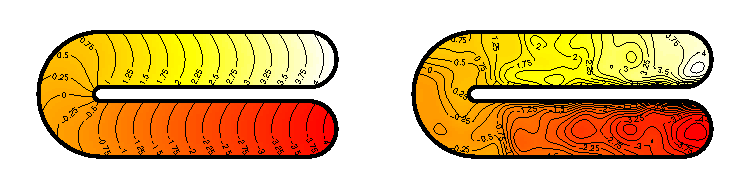
\includegraphics{intro/figs/ramsay-leak.pdf}\\
\caption{An example of leakage. A thin plate regression spline was fit to data sampled from the function on the left, the model smooths across the gap in the middle of the domain (right.)}
\label{leakage}
\end{figure}

The problem of leakage arises because of the way in which the smoother measures how near objects are to one another. Most smoothing techniques use the Euclidean metric to measure the distance between data. Clearly though, this approach is flawed: biological populations do not conform to Euclidean geometry in their movement patterns and hence their observed positions will reflect this. Just as whales do not uniformly distribute themselves across sea and glacier, fish do not lay their eggs on land. Natural and man-made barriers carve up the landscape (and seascape), partitioning biological populations; spatial models should take this into account.

The response may be smooth, just not necessarily over $\mathbb{R}^2$ (\cite{wangranalli}). Modelling the structure of the domain correctly by embedding the extra information relating to the shape of the boundary (whether this be implicitly or explicitly) allows models to represent this smoothness.

\subsection{Ramsay's horseshoe function as a benchmark for finite area smoothing}

\label{ramsayfunc}

\citeb{ramsay} proposes a function which can be used to benchmark new approaches to 2-dimensional smoothing. The function takes the form of a horseshoe shape which is flat across the domain has a gradient along the domain's major axis. This can be seen in \fig{orig-fs}. \citeb{soap} modifies the test function by adding curvature across the minor axis of the shape (left plot in figure \ref{leakage}). This was added in order to avoid the horseshoe function lying in the nullspace of their model's penalty, making the problem too easy for their method. It is the second shape that will be used for simulations here and shall be referred to as the \emph{Ramsay horseshoe} throughout.

% original horseshoe from Ramsay's paper
\begin{figure}
\centering
% trim order l b r t
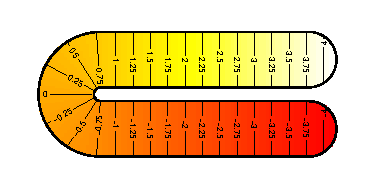
\includegraphics{intro/figs/orig-fs.pdf}\\
\caption{The horseshoe function as it appeared in \citeb{ramsay}.}
\label{orig-fs}
\end{figure}

As mentioned above, when the smoothing problem is specified in terms of Euclidean distance, the model takes the distance between the points in the two arms of the horseshoe as the distance over the gap in-between them, rather than the distance along the major axis of the shape. This causes the high function values from one side to contaminate the other side (and the low to contaminate the high).
		
\subsection{Previous approaches to leakage}
\label{intro-leakageapproaches}

The cause of leakage can be characterized in two ways: either the smooth does not respect the boundary of the domain, or the smooth does not take into account the geometry of the domain (in particular with regard to the distance between points within the domain). Previous work in this area has been to combat leakage along these two lines. Work of \citeb{ramsay} and \citeb{soap} both use a partial differential equation (PDE) boundary condition approach to try to prevent leakage, whereas \citeb{wangranalli} and \citeb{eilerstalk} modify the way that inter-point distances are measured in order to avoid smoothing across boundaries. These four main works are now summarized.

\begin{enumerate}
\item \citeb{ramsay} proposes finite element $L$-splines (FELSPLINEs). The $L$-spline penalty is similar to the one in (\ref{intro-2d-objfcn}):
\be
\int_\Gamma (L_p f)^2 \text{d}\mathbf{x}.
\ee
Integration is performed over $\Gamma$ (the domain over which the smoothing is to take place) and $L_p$ is a roughness operator defined as:
\be
L_p=\Delta^p+c_{p-1}\Delta^{p-1}+\dots+c_1\Delta+c_0I.
\ee
Here $I$ is the identity operator, the $(c_0,\dots, c_p)$ are constants and $\Delta$ is the Laplacian (sum of second derivatives with respect to $x_1$ and $x_2$). This can be thought of as simply replacing the $P$ operator in (\ref{intro-2d-objfcn}) and changing the integration domain. 

In order to find $f$ Ramsay takes a finite element approach. First triangulating the domain, then constructing a set of bivariate quadratic polynomial basis functions over each triangle, specifying that there be continuity over the edges of the triangles. By taking the FELSPLINE objective function and transforming it into a variational form (as one would for a PDE), the approximation to the minimizer of the objective function is found.

Since the triangulation and hence the penalty of the FELSPLINE is only calculated over the domain, and the continuity is specified over neighbouring cells, the method prevents leakage. However, although FELSPLINE does not exhibit leakage on the original horseshoe (\fig{orig-fs}), in practice the model makes unrealistic physical assumptions. The boundary conditions of FELSPLINE specify that the gradient is zero, along normals to the boundary. This is not always physically realistic. \citeb{soap} show that by modifying the test function on horseshoe domain (see \secref{sc-alt-horsehoe}), the FELSPLINE performance begins to falter.

FELSPLINE does not offer a realistic physical model and is therefore not a viable solution to the finite area smoothing problem in general.

\item \citeb{wangranalli} adopt a ``within-area distance'' formulation for thin plate splines. They choose to use the geodesic distance between two points, that being the shortest path within the domain. This gives a definition of how near objects are in the domain. The within-area distances are used in the radial basis functions in place of the Euclidean norm (\secref{GAMtprs}).

To calculate the distances, Wang and Ranalli first create a complete, weighted, undirected, graph ($G$, say) with a data point at each vertex and the distance between each pair of vertices as the weights on the edges. They then find the restricted graph of $G$, $G_k$, in which each vertex is only connected to its $k$ nearest neighbours. With this new, restricted graph the geodesic distances between each pair of vertices can be calculated using Floyd's algorithm (\cite{Floyd}).

As the authors point out, the quality of the approximation is dependent on the size of the data set and its density. At low densities the estimated geodesic distance will tend towards the Euclidean, at high densities the approximation tends, asymptotically toward the true geodesic distance (\cite{bernstein}). Even if  dense enough data were available, the method will be rather slow since Floyd's algorithm is cubic in the number of vertices (the size of the data set). 

Taking these points into account, Wang and Ranalli's approach appears cumbersome, slow and dependent on dense data.

\item The soap film smoother (\cite{soap}) uses a rather simple physical model to prevent leakage from occurring. First, consider the domain boundary to be made of wire, then dip this wire into a bucket of soapy water, you will then have a soap film in the shape of your boundary. Consider the wire to lie in the $x_1-x_2$ plane and the height of the soap film at a given point to be the functional value of the model (i.e. in the $z$ direction). This film is then distorted smoothly by moving it toward the data, while minimising the surface tension in the film.

Fitting a model using the soap film smoother consists of first finding a set of basis functions which are solutions to a series of partial differential equations (PDEs) which define the film. Since these functions arise from PDE with boundary conditions, the resulting functions respect those boundary conditions (which can be estimated from the data or set to some known values), by default. 

Although mathematically elegant, the soap film smoother is a rather complex and computationally expensive model (since the series of PDEs must be solved every time). One must also pick knots for the soap film smoother to use, introducing an element of arbitrariness into the fitting process. The model also treats the boundary as something special, it is not clear that this is always appropriate (in particular thinking of ocean-based studies where some of the boundaries are coastlines but others are essentially arbitrary).

Although not perfect, the soap film smoother will be used throughout the thesis a the ``gold standard'' against which the methods proposed herein will be measured. The soap film was chosen over the other methods above since it is already implemented in the \textsf{R} package \texttt{soap} (unlike GLTPS, which does not have an easily available implementation) and it does not have any obvious major technical flaw (like the unrealistic physical assumptions that FELSPLINE makes).

Chapter \ref{chap-it} gives the technical details relating to the construction of the basis. The chapter also further illustrates the soap film smoother via a case study showing its use as the spatial part of a spatiotemporal model for the incidence of resident foreigners in Italy. 

\item An alternative approach to treating the boundary as something special is to transform the space in which the points lie to a different domain which is more suitable for smoothing. For example, with Ramsay's horseshoe, it seems intuitive to simply bend the horseshoe into a long strip and then smooth on that domain.

Indeed, \citeb{eilerstalk} proposed using the \textit{\sch\ transform} for this very purpose (the author independently came to the idea in 2008). The basic idea is to find a function that takes points in the domain the data lie in and maps them to another domain in which smoothing is easier. Using the \sch\ transform for smoothing will be investigated in chapter \ref{chap-sc}.

Outside of the smoothing spline and GAM literature, transformation-based methods have also been suggested, in particular, when using a kriging approach (see \citeb[pp. 425-430]{MASS} for a concise introduction, \citeb{schabenberger} or \citeb{diggle} for a thorough treatment). Kriging consists of modelling the spatial correlation between points via the \textit{semivariogram} and a spatial trend via a mean function (similar to the linear predictor in the smoothing case, although there are flavours of kriging where the mean is considered constant and/or known). Semivariogram models assume that the correlation between points is related to the distance between the points but not their position (this is known as \textit{stationarity}, and comes in varying degrees, \citeb[pp. 42-44]{schabenberger}). When the boundary of the domain has a complex shape, the correlation between points is likely to vary with distance within the domain rather than the Euclidean distance between points. Simply substituting within-area distances into the semivariogram will lead to an invalid semivariogram (\secref{gds-krig}; \cite{curriero})

Several authors have suggested the use of some kind of transformation of the data points in space in order to maintain stationarity by approximating within-area distances with equivalent Euclidean distances via \textit{multidimensional scaling} (\cite{mdskrig}; \cite{crabkrig}; \cite{curriero}). The use of multidimensional scaling to project these distances ensures that the semivariogram remains positive or conditionally negative definite (which is required to have a valid semivariogram, \citeb{curriero}).

%Although not specifically designed to deal with leakage issues (although leakage manifests itself as a breakdown of stationarity in a kriging context), several authors have suggested the use of some kind of transformation of the data points in space in order to maintain stationarity by approximating within-area distances with equivalent Euclidean distances via \textit{multidimensional scaling} (\cite{mdskrig}; \cite{crabkrig}; \cite{curriero}). 

Using multidimensional scaling as a transformation of a spatial domain is investigated in chapters  \ref{chap-mds} and \ref{chap-gds}. A comparison between the geostatistical implementations and the methods developed in this thesis is given in \secref{gds-krig}, once the proposed methods have been fully explained.
\end{enumerate}

Creating some kind of mapping between the space in which the data lies and the space in which conventional smoothers perform well is convenient. Relying on existing, tested methodology is clearly appealing. Transformation-based approach also benefit from not treating the boundary as a special in the basis setup. The properties that such a mapping would require to be useful for smoothing will be investigated in subsequent chapters.

Chapters \ref{chap-sc}, \ref{chap-mds} and \ref{chap-gds} investigate the combination a transformation of space and conventional smoothers to solve the problem of leakage in finite area smoothing. The next chapter attempts to solidify the concepts presented so far (smoothing, penalties, leakage, tensor products) as well as highlight some of the potential pitfalls when modelling complex data. The chapter applies a spatiotemporal model of legal immigrants in Italy using a tensor product of a soap film smoother basis (for space) and a cubic spline basis (for time).